%----------------------------------------------------------------------------
\chapter{Kódolási eszközök}\label{sect:CodeTool}
%----------------------------------------------------------------------------

\hspace{2mm} A feladatomhoz fontos volt a megfelelő kódolási eszközök felmérése és megismerése, ebben a fejezetben ezt részletezem. 

\section{HTML, CSS}
\hspace{2mm} Régebben komoly problémát jelentett, hogy a szabványok nem megfelelő megfogalmazásából adódóan a böngészők eltérően implementálták a dolgokat, így rendszeres megjelnésbeli külnbségek merültek fel. Ez persze az évek során nagyon sokat finomodott, míg végül a World Wide Web Consortium (W3C) lefektetett egy úgy látszik megfelelően magalapozott szabványt a HTML5-tel. Ez a szabvány egységesítette az előtte már kétirányba elhúzódó (XHTML és HTML4) szabványokat. A másik nagy előnye az volt ennek a szabványnak, hogy lehetőséget biztosított a modern kliens oldali fejlesztésnek (Canvas) és az oldal strukturáltáságát is javította renget új elem bevezetésével (article, nav stb...).

A HTML alapvetően csak az oldal logikai struktúrájának leírását szolgálja, és ez a tulajdonsága az évek alatt nem is változott. Nem képes a komplexebb megjelenítési feladatok ellátására, csak az egyes felületelemeket tudjuk megadni ún. tagekkel deklaratív módon.

Mivel a HTML-el nem tudjuk érdemben befolyásolni a lap kinézetét megszületett CSS (Cascading Style Sheets). A CSS segítségével gyakorlatilag minden HTML elemet akár külön-külön meg tudunk formálni, olyanná amilyenre szeretnénk. A CSS szabványok terén még nagyobb volt a káosz, mint a HTML-eknél, főleg amiatt, hogy gyorsan mentek végbe a változások, szerencsére a CSS szabványait végül a CSS3 egybegyúrta.  

%----------------------------------------------------------------------------
\section{Javascript, Typescript}
\hspace{2mm} A jelenleg legnépszerűbb nyelv a webes alkalmazások készítésére a Javascript. Gyakorlatilag minden böngésző támogatja semmilyen beépülő modulra nincs szükség. A böngészők a javascript belső implementációját igyekeztek egységeséteni a szabványnak megfelelően, továbbá a hatékonyság érdekében rengeteget könnyítettek a fejlesztéseken, egyre jobb memóriakezelést alkalmaztak és a böngészőmotorok fel lettek szerelve a töbszálú futás lehetőségével is így nagyobb alkalmazások is könnyen tudnak rajtuk futni.

Magát a nyelvet 1997-ben ECMAScript néven szabványosították először. Az objektumorientált nyelvek családjába tartozik, azon belül is a prototipusos nyelvek közé. Ez a gyakorlatban annyit tesz, hogy nem rendes osztályok vannak a nyelvben, amiket aztán példányosítunk, hanem minden objektum egy prototipus objektum "lemásolásával" jön létre. Ez a nyelv és az egyes objektumok nagyon szabad kezelését teszi lehetővé, gyakorlatilag nyílt objektumaink vannak, amiket szabadon felruházhatunk új attribútumokkal metódusokkal a fejlesztés dinamikus és gyors lehet.

\begin{figure}[!ht]
\centering
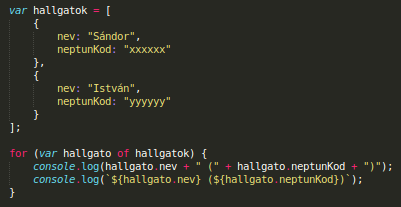
\includegraphics[width=0.5\textwidth, keepaspectratio]{figures/javascript.png}
\caption{Egy Javascript objektum} 
\label{fig:JS}
\end{figure} 

A \figref{JS}-es ábra mutat egy példát egy ilyen objektum létrehozására. Fontos megemlíteni, hogy a JavaScript változói dinamikusak, azaz csak futási időben kapnak értéket, és típusuk is csak ekkor derül ki, sőt akár változhat is. Egy további érdekessége a nyelvnek, hogy minden objektumként viselkedik még a függvények is, így értelmezve van mindennél a \textit{this} kulcsszó.

A fenti prototípusosság azonban nagy hátrányt is jelenthet a fejlesztőknek, ugyanis semmilyen megkötés vagy követelés nincsen így arra, hogy az egy objektum milyen tulajdonságokkal rendelkezzen futási időben. Ez nagyon sok kényelmetlenséget okoz a hívó félnek és hívottnak is, ugyanis fel kell készülni, hogy az adott metódus bármilyen paramétert megkaphat, nem köthetjük ki a típusát. Ennek orvoslására rengeteg megoldás született, melyek más-más módokon segítik a fejlesztést. Én ezek közül a TypeScriptet választottam mely egy a Microsoft által fejlesztett scriptnyelv. \cite{Typescript}
A fejleszése során előre készültek az ECMAScript2016-os szabványra, így az átállás nem lesz nehéz. Ez a nyelv gyakorlatilag egy plusz réteget biztosít a Javascript főlé, melyben garantálva van a típusosság. A legjobb tulajdonsága, hogy plain JavaScriptre fordul, azaz egy fordító egy az egyben JavaScript kódot állít elő a TypeScript kódunkból, gyakorlatilag semmilyen böngésző támogatásra nincs szükségünk. 

\begin{figure}[!ht]
\centering
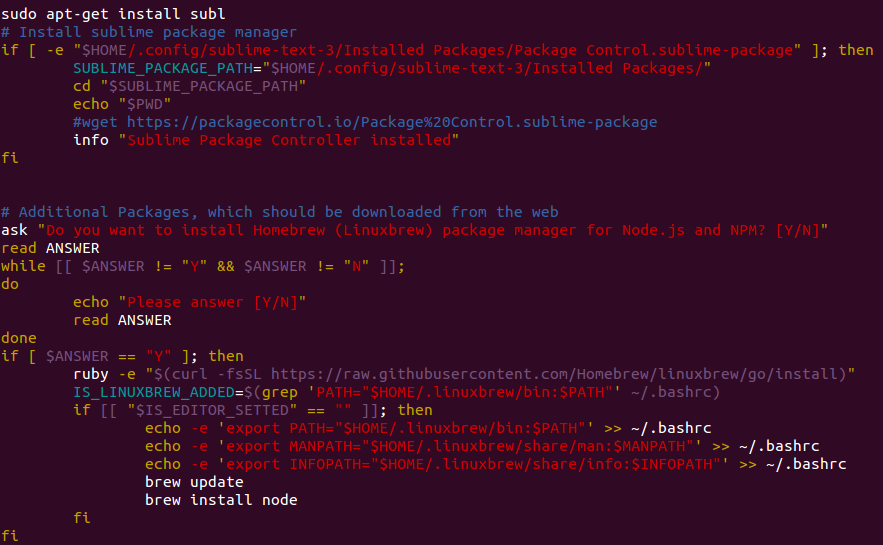
\includegraphics[width=\textwidth, keepaspectratio]{figures/typescript1.png}
\caption{Typescript installáció} 
\label{fig:TS1}
\end{figure} 

A TypeScript fordításához szükség van a NodeJS, npm telepítésére. Ezen kívül a fejlesztő környezet is kérdéses lehet, ugyanis egyre több jó szövegszerkesztő van amiben van TypeScript támogatás. 
A legjobbak talán a Visual Studio Code, a Webstorm, az Atom, az Eclipse és a NetBeans, de van már vimben és Sublime Text-ben is támogatás. A telepítések automatizálására írtam egy shell scriptet (\figref{TS1}), a fejlesztőkörnyezetnek pedig a Sublime Text-et választottam (\figref{TS2}, ennek az editornak van külön package controllerje, amit a script szintén felrak ezután már csak a TypeScript packaget kell letölteni és kész is a támogatás. 

\begin{figure}[!ht]
\centering
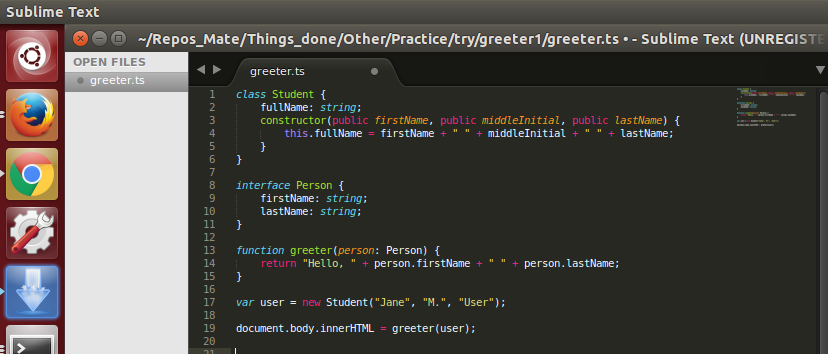
\includegraphics[width=\textwidth, keepaspectratio]{figures/typescript2.png}
\caption{Typescript osztály és interfész Sublime Text-ben} 
\label{fig:TS2}
\end{figure} 

A \figref{TS2}-es ábrán látható, egy egyszerű osztály és interfész. Az egyes osztályokat a \textit{module} kulcsszóval lehet csoportokba rendezni, ami hasonló a C++ namespace-eihez. Ha az osztály elé odarakjuk \textit{export} kulcsszót, akkor az az osztály kívülről is elérhetővé válik. Ezeken kívül már hasonló a szintaktika, kell konstruktor és lehet public vagy private változókat megadni, annyi talán a különbség, hogy a változó neve után írjuk a típust kettősponttal elválasztva. Az interfaceken keresztül metódusok érhetők el. A fordítás során keletkezik pár segéd fájl, ilyen pl. a map fájl mely a debuggernek segít a JavaScript TypeScript kódrészletek összepárosításához. 

Meg kell említeni, hogy a nyelv rengeteg újszerű nyelvi elemet tartalmaz. Ilyen például az async/await mely az aszinkron műveletek kezelésében segít, az enum felsorolás típus, az import kulcsszó más fájlokra hivatkozáshoz de ide sorolhatjuk az any kulcsszót is, amivel dinamikusosan típusos változót készíthetünk Typescriptben is.

Ennek a nyelvnek a legnagyobb előnye, hogy a fentiek miatt jól struktúrálható kódot készíthetünk.
%----------------------------------------------------------------------------
\section{Canvas, KonvaJS}

Az alkalmazáson belül a diagram megjelenítésére több lehetőségem volt. Meg lehetett volna oldani csak HTML-el azonban ez a megoldás nem támogatja a különleges alakzatok (nem téglalap) megjelenítését, így ezt hamar elvetettem. Két lehetséges módszer maradt az SVG és a Canvas. Mindkettő megfelelt a feladat elvárásainak, azonban a Canvas mellett döntöttem, mivel ez egy újabb fejlődőbb technika több lehetőséggel. A Canvas pixelpontos rajzolást tesz lehetővé és bármilyen alakzatot könnyedén meg lehet vele rajzolni. A nagy hátránya az, hogyha megrajzoltunk egy alakzatot, akkor arra utána nem lehet már hivatkozni, az alakzatok között semmilyen kommunikáció nincs, nekünk kell elvégezni a nyilvántartást

Utánajárva a problémának az alakzatok közötti eseménykezelést a KonvaJS függvénykönyvtár segítségével oldottam meg. \cite{KonvaJS} Több lehetőségem is volt, ez a függvénykönyvtár a már elavult KineticJS keretrendszerből fejlődött ki, és egy fél éve a KineticJS keretrendszer fejlesztője is ezt jelölte meg alternatívaként, azóta kijött 2016 március 30-án a ConcreteJS keretrendszer is, ám ez még elég fiatal, sok hasznos funkciója van, de még a KonvaJS melett maradtam.

\begin{figure}[!ht]
\centering
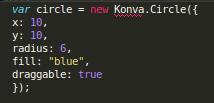
\includegraphics[width=0.4\textwidth, keepaspectratio]{figures/konva.png}
\caption{Egy egyszerű kör rajzolása KonvaJS segítségével} 
\label{fig:Konva}
\end{figure} 

A függvénykönyvtár segítségével az egyes alakzatok csoportosíthatók. A \figref{Konva}-es ábra mutatja egy egyszerű kör rajzolását, egy sima API-n keresztül létre lehet hozni az alakzatot. Nagy segítség még a fejlesztéshez, hogy készült hozzá Typescript interfész is leírással.